%!TEX root =../quadrotorbook.tex

\chapter{Optical Flow and Feature Tracking}
\label{chap:optical_flow}

This chapter discusses two related algorithms.  The first, discussed in Section~\ref{sec:optical_flow}, is the computation of optical flow at a pixel.  The optical flow field can then be computed by finding the optical flow at a set of pixel locations.  The second algorithm discussed in Section~\ref{sec:klt_feature_tracking} is the KLT feature tracking algorithm, that uses an iterated computation of optical flow, to find how specific features have moved from one frame to the next.  Section~\ref{sec:klt_feature_tracking_with_imu} describes an extension of the KLT algorithm that uses the IMU to enable tracking across large camera motion, as might occur during aggressive flight.  The final section in this chapter, Section~\ref{sec:optical_flow_guidance} describes simple guidance algorithms for multirotors that use the optical flow field to maneuvers through canyons and around obstacles.

%-----------------------------------------------
\section{Levenberg-Marquardt (LM) Optimization}
\label{sec:LM_optimization}

\rwbcomment{Probably put this somewhere else.  Maybe in the preliminaries chapter.}

The Levenberg-Marquart (LM) algorithm is a standard technique for solving nonlinear least squares problems of the form
\[
\beta^\ast = \arg\min r(z, \beta)^\top r(z, \beta),
\]
where $z\in Z$ is a known data vector, $\beta \in B$ is a parameter vector, and $r:Z\times B\to \mathbb{R}^N$ is a residual vector to be minimized.  
The optimization problem is solved by iteratively incrementing $\beta$ by a small $\delta$ in a direction that decreases the squared residual
\[
S(\beta) = r(x, \beta)^\top r(z, \beta).
\]

Using the approximation 
\[
r(z, \beta+\delta) \approx r(z, \beta) + J(z, \beta)\delta,
\]
where 
\[
J(z, \beta) \defeq \frac{\partial r}{\partial \beta} (z, \beta)
\]
is the Jacobian of $r$ with respect to the parameters $\beta$, we get that
\[
S(\beta+\delta) \approx [r(z, \beta) - J(z, \beta)\delta]^\top [r(z, \beta)- J(z, \beta)\delta].
\]
Taking the partial of $S(\beta+\delta)$ with respect to $\delta$ and setting equal to zero gives
\begin{equation}\label{eq:gauss-newton}
J^\top r = J^\top J \delta.
\end{equation}
Solving for $\delta$ from this equation results in the Gauss-Newton optimization method.  In contrast, gradient descent replaces the right hand side of Equation~\eqref{eq:gauss-newton} by $\lambda\delta$, where $\lambda$ is a scalar. The LM algorithm is a hybrid between Gauss Newton and gradient descent, requiring $\delta$ to satisfy
\begin{equation}\label{eq:LM_lambda}
J^\top r = (J^\top J + \lambda I) \delta.
\end{equation}
The general LM optimization algorithm is therefore given by the iteration
\begin{equation}\label{eq:general_lm_alg}
\beta_{\ell+1} = \beta_\ell + \delta_\ell,
\end{equation}
where
\[
\delta_\ell = \left[J(z,\beta_\ell)^\top J(z,\beta_\ell) + \lambda_\ell I\right]^{-1} J(z,\beta_\ell)^\top r(z, \beta_\ell),
\]
where $\lambda_\ell$ is selected at each iteration to ensure that the residual $r(z, \beta)$ decreases.

%------------------------------------------------------------
\section{Optical Flow}
\label{sec:optical_flow}

Suppose that a camera attached to a multirotor collect image $I_k$ at time $k$ and image $I_{k+1}$ at time $I_{k+1}$, and suppose that $\mbf_0 = (m_x, m_y)^\top$ is a pixel of interest in image $I_k$.  The objective is to find the corresponding pixel in image $I_{k+1}$ using only image data.  We assume that lighting qualities in the scene do not change between images $I_k$ and $I_{k+1}$.  

Let $\deltabf = (\delta_x, \delta_y)^\top$ be a small change in pixel locations, then the objective is to find $\deltabf$ to minimize the residual
\begin{equation}\label{eq:optical_flow_1}
r(I_k, I_{k+1}, \mbf_0, \deltabf) = I_{k+1}(\mbf_0+\deltabf) - I_k(\mbf_0),
\end{equation}
where $\mbf_0+\deltabf$ is the pixel location in the new image of the feature located at $\mbf_0$ in the old image.  It turns out that finding the optical flow at a single pixel under-determined and susceptable to noise  Therefre, the residual function is modified to minimize the intensity values over a window surrounding $\mbf_0$ as
\begin{equation}\label{eq:optical_flow_1}
r(I_k, I_{k+1}, \mbf_0, \deltabf) = \begin{pmatrix} \left(I_{k+1}(\xbf_1+\deltabf) - I_k(\xbf_1)\right) \\
\vdots \\
\left(I_{k+1}(\xbf_n+\deltabf) - I_k(\xbf_,)\right)
\end{pmatrix}
\end{equation}
where $\xbf_1, \dots, \xbf_n$ are the pixels in the window $W(\mbf_0)$ around the pixel $\mbf_0$.  


%The solution is perhaps easiest to derive in continuous time.  Let $I(\mbf_0, t)$ be the image intensity at $\mbf_0$ at time $t$, then equation~\eqref{eq:optical_flow_1} can becomes
%\[
%I(\mbf_0 + \deltabf dt, t+dt) = I(\mbf_0, t).
%\]
Following the previous section and taking the Taylor series expansion of the residual gives
\begin{align*}
r(I_k, I_{k+1}, \mbf_0, \deltabf) &\approx \begin{pmatrix} I_k(\xbf_1) + \frac{\partial I_k}{\partial t}(\xbf_1) + \frac{\partial I_k^\top}{\partial \mbf}(\xbf_1)\deltabf + H.O.T. - I_k(\xbf_1) \\
\vdots \\
I_k(\xbf_n) + \frac{\partial I_k}{\partial t}(\xbf_n) + \frac{\partial I_k^\top}{\partial \mbf}(\xbf_n)\deltabf + H.O.T. - I_k(\xbf_n)
\end{pmatrix} \\
	&\approx \begin{pmatrix} \frac{\partial I_k}{\partial t}(\xbf_1) + \frac{\partial I_k^\top}{\partial \mbf}(\xbf_1)\deltabf \\
	\vdots \\
	\frac{\partial I_k}{\partial t}(\xbf_n) + \frac{\partial I_k^\top}{\partial \mbf}(\xbf_n)\deltabf
	\end{pmatrix}
\end{align*}
where the computation of $\frac{\partial I}{\partial \mbf}$ is given in Equation~\eqref{eq:image_gradient}, and where 
\[
\frac{\partial I_k}{\partial t}(\xbf_i) \approx I_{k+1}(\xbf_i) - I_k(\xbf_i),
\]
where the units of $\frac{\partial I_k}{\partial t}$ is intensity/sample, the units of $\frac{\partial I_k}{\partial \mbf}$ is intensity/pixels, and the units of $\deltabf$ is pixels/sample.  

The optical flow problem can now be stated as the problem of finding the optical flow vector $\deltabf$ to minimize the squared error of the residual function.  
Letting $S = r^\top r$ we get 
\begin{align*}
S(I_k, I_{k+1}, \mbf_0, \deltabf) &= \sum_{\xbf\in M(\mbf_0)} \left(\frac{\partial I_k}{\partial t}(\xbf) + \frac{\partial I_k^\top}{\partial \mbf}(\xbf)\deltabf\right)^\top \left(\frac{\partial I_k}{\partial t}(\xbf) + \frac{\partial I_k^\top}{\partial \mbf}(\xbf)\deltabf\right) \\
&= \deltabf^\top \left(\sum_{\xbf\in M(\mbf_0)}\frac{\partial I_k}{\partial \mbf}(\xbf)\frac{\partial I_k^\top}{\partial \mbf}(\xbf)\right) 
	+ 2\left(\sum_{\xbf\in M(\mbf_0)}\frac{\partial I_k}{\partial t}(\xbf)\frac{\partial I_k}{\partial \mbf}(\xbf)\right)^\top \deltabf 
	+ \left(\sum_{\xbf\in M(\mbf_0)}\frac{\partial I_k^2}{\partial t}(\xbf) \right) \\
&= 	\deltabf^\top G(\mbf_0) \deltabf + 2b^\top(\mbf_0) \deltabf + c,
\end{align*}
where $G(\mbf_0)$ is given in Equation~\eqref{eq:G_mbf}m, and 
Define 
\begin{align*}
b(\mbf_0) &\defeq \left(\sum_{\xbf\in W(\mbf_0)} \frac{\partial I}{\partial\mbf}(\xbf) \frac{\partial I}{\partial t}\right), \\
c(\mbf_0) &\defeq \sum_{\xbf\in M(\mbf_0)}\frac{\partial I_k^2}{\partial t}(\xbf).
\end{align*}
Taking the partial of $S$ with respect to $\deltabf$ and setting equal to zero gives
\[
\delta = G^{-1}(\mbf_0) b(\mbf_0).
\] 
%
%
%
%
%Equation~\eqref{eq:optical_flow_2} is one equation in two unknowns. Since the computation of image gradients is susceptible to noise, the optical flow vector $\deltabf$ is found as the solution to a least squares problem, where Equation~\eqref{eq:optical_flow_2} is evaluated on a window centered at $\mbf_0$.  Let $\xbf_1, \dots, \xbf_n$ be the pixels in the window $W(\mbf_0)$, then the optical flow vector $\deltabf$ is the least squares solution to 
%\[
%\begin{pmatrix}
%\frac{\partial I^\top}{\partial\mbf}(\xbf_1) \\
%\vdots \\
%\frac{\partial I^\top}{\partial\mbf}(\xbf_n)
%\end{pmatrix} \deltabf
%+ \begin{pmatrix}
%\frac{\partial I}{\partial t}(\xbf_1) \\
%\vdots \\
%\frac{\partial I^\top}{\partial t}(\xbf_n).
%\end{pmatrix} = 0
%\]
%Multiplying both sides by 
%\[
%\begin{pmatrix} 
%\frac{\partial I}{\partial\mbf}(\xbf_1), &
%\cdots, &
%\frac{\partial I}{\partial\mbf}(\xbf_n)
%\end{pmatrix}
%\]
%gives
%\begin{equation}\label{eq:optical_flow_3}
%\left(\sum_{\xbf\in W(\mbf_0)} \frac{\partial I}{\partial\mbf}(\xbf)\frac{\partial I^\top}{\partial\mbf}(\xbf)\right)\deltabf 
%+ \left(\sum_{\xbf\in W(\mbf_0)} \frac{\partial I}{\partial\mbf}(\xbf) \frac{\partial I}{\partial t}\right) = 0.
%\end{equation}
%Define 
%\[
%b(\mbf_0) \defeq \left(\sum_{\xbf\in W(\mbf_0)} \frac{\partial I}{\partial\mbf}(\xbf) \frac{\partial I}{\partial t}\right),
%\]
%and note that first matrix in Equation~\eqref{eq:optical_flow_3} is equal to $G(\mbf_0)$ in Equation~\eqref{eq:G_mbf}.  Therefore, the optical flow vector at pixel $\mbf_0$ is given by\cite{MaSoattoKoseckaSastry03}
%\begin{equation}\label{eq:optical_flow_4}
%\deltabf(\mbf_0) = - G^{-1}(\mbf_0) b(\mbf_0).
%\end{equation}
Of course this equation requires that $G(\mbf_0)$ is full rank, i.e., $\rank{G(\mbf_0)}=2$.  If $\mbf_0$ is a \texttt{goodfeaturetotrack} then the eigenvalues are both positive and $G(\mbf_0)$ is full rank.  However, for pixel locations that do not have gradients in both directions, $G(\mbf_0)$ will lose rank and the optical flow vector cannot be computed at that point.  

As described in the previous section, the Gauss-Newton iteration gives
\[
\mbf_{\ell+1} = \mbf_\ell + G^{-1}(\mbf_\ell) b(\mbf_\ell).
\]

The method described above assumes that the intensity at pixel $\mbf_0$ moves a small distance that is at least contained in the window $W(\mbf_0)$, and the method can fail for large motions.  
\rwbcomment{Need to describe image pyramids}.
One method for compensating for this problem is to compute the a set of image pyramids and to compute the optical flow vector on a lower resolution image in the pyramid, where small optical flow vector now correspond to larger motions in the image.  The optical flow algorithm is then computer at higher resolutions using the seed from the lower resolution image.  

The \texttt{openCV} function \texttt{calcOpticalFlowPyrLK()} computes the optical flow at a set of points passed into the function.
\sidenote{\href{https://docs.opencv.org/3.4/d4/dee/tutorial_optical_flow.html}{\texttt{openCV code example}}.}

Our discussion to this point has used uncalibrated pixel coordinates $\mbf = (m_x, m_y)^\top$.  Equation~\eqref{eq:optical_flow_4} gives the optical flow vector and can be written as
\[
\dot{\mbf} = (\dot{m}_x, \dot{m}_y)^\top = \deltabf(\mbf).
\]
In calibrated normalized pixel coordinated we have
\[
\bar{\epsilonbf} = K_c^{-1}\bar{\mbf} = K_c^{-1}\begin{pmatrix} m_x \\ m_y \\ 1 \end{pmatrix}.
\]
Therefore, the optic flow vector in calibrated normalized pixel coordinates is given by
\begin{align*}
\dot{\bar{\epsilonbf}} &= \begin{pmatrix} \dot{\epsilon}_x \\ \dot{\epsilon}_y \\ 0 \end{pmatrix} \\ 
&= K_c^{-1} \begin{pmatrix} \dot{m}_x \\ \dot{m}_y \\ 0 \end{pmatrix} \\ 
&= K_c^{-1} \dot{\bar{\mbf}},
\end{align*}
and the units of $\dot{\bar{\epsilonbf}}$ are $\text{seconds}^{-1}$.

%------------------------------------------------------------
\section{KLT Feature Tracking}
\label{sec:klt_feature_tracking}.

The KLT feature tracking method, which was first reported in (Lucas \& Kanade)~\cite{LucasKanade81}, is different than the optical flow method described in Section~\ref{sec:optical_flow} in two ways. 
\marginnote{KLT stands for "Kanade, Lucas, Tomasi" and represents the fact that the method explicitly uses Shi-Tomasi features.}
First, the optical flow vector is computed at a good-feature-to-track.  Therefore, it has already been determined that $G(\mbf)$ is invertible.  The second difference is that the optical flow vector is iteratively refined, rather than simply solving Equation~\eqref{eq:optical_flow_4} one time.  

Beginning with the good feature point $\mbf$, Equation~\eqref{eq:optical_flow_4} is solved to find the estimated new pixel location 
\[
\mbf_1 = \mbf + \deltabf(\mbf) = \mbf + G^{-1}(\mbf)b(\mbf).  
\]
The gradient data $G$ and $b$ are then evaluated at $\mbf_1$ and the process is repeated interatively.  The KLT feature tracking algorithm can be described using the equation
\[
\mbf_{\ell+1} = \mbf_\ell + G^{-1}(\mbf_\ell)b(\mbf_\ell)  
\]

The \texttt{openCV} implementation of \texttt{calcOpticalFlowPyrLK()} iterative computes the optical flow vector at specified points.  When \texttt{calcOpticalFlowPyrLK()} is used in conjunction with \texttt{goodFeaturesToTrack}, the resulting algorithm is the KLT feature tracker.


%------------------------------------------------------------
\section{KLT Feature Tracking with IMU}
\label{sec:klt_feature_tracking_with_imu}

In this section we address the question of whether an IMU can be used to assist optical flow algorithm.  The basic idea is the seed the iteration
\[
\mbf_{\ell+1} = \mbf_\ell + G^{-1}(\mbf_\ell)b(\mbf_\ell)
\]
with a best guess from the IMU, rather than the feature location $\mbf_0$.  

\rwbcomment{come back to this.  The notation is not quite adequate since $I_t$ has to be computed at both $\mbf_0$ and $\mbf_\ell$.}


In this section, we address the issue of initializing the optical flow algorithm  optimization given in Algorithm~\ref{alg:LM_optimization}.  We are particularly interested in the robotic situation where an IMU, synchronized to the camera, is available to resolve the scale ambiguity.  We will also discuss the case where IMU measurements are not available.  The discussion in this section follows in some respects, the development in~\cite{ForsterCarloneDellaert17}.  

For the sake of clarity, in this section we will again explicitly specify the different coordinate frames.  Let $R_k^I\in SO(3)$ be the rotation from the camera frame at time $k$, $\mathcal{F}^k$ to the inertial frame $\mathcal{F}^I$, and let $\xi_{k/I}^k$ and $v_{k/I}^k$ be the position and velocity of the camera at time $k$ relative to the inertial frame, expressed in the camera frame $\mathcal{F}^k$, let $a_{k/I}^k$ be the measured specific acceleration of the camera expressed in $\mathcal{F}_k$, and $\omega_{k/I}^k$ be the measured angular velocity of the camera relative to the inertial frame, as expressed in the camera frame $\mathcal{F}^k$, where we have assumed that the IMU biases are known and have been removed from the measurements.  Then the kinematics for the camera are given by
\begin{align}
\dot{R}_k^I &= R_k^I \left(\omega_{k/I}^k\right)_\times \notag \\
\dot{v}_{k/I}^k &= R_k^{I\top} g^I + a_{k/I}^k, \label{eq:kinematics} \\
\dot{\xi}_{k/I}^k &= v_{k/I}^k  \notag
\end{align}
where $g^I$ is the gravity vector in the inertial frame.  Let $T_s$ be the sample period of the IMU, and assume that there are $m$ IMU samples between camera frames.  We will use the notation $\kappa_0, \kappa_1, \kappa_2, \dots, \kappa_m$ to denote the intermediate sample from $k-1$ to $k$, implying that the time instance $\kappa_0$ corresponds to the time at image frame $k-1$, and $\kappa_m$ corresponds to the time at image frame $k$.  Then, integrating over one sample of the IMU and assuming that the measurements are constant over the sample period, we get
\begin{align*}
R_{\kappa_{i+1}}^I &= R_{\kappa_i}^I \exp\left((\omega_{\kappa_i/I}^{\kappa_i})_\times T_s \right) \\
v_{\kappa_{i+1}/I}^{\kappa_{i+1}} &= R_{\kappa_i}^{\kappa_{i+1}}v_{\kappa_i/I}^{\kappa_i} + R_{\kappa_{i+1}}^{I\top} g^I T_s +R_{\kappa_i}^{\kappa_{i+1}} a_{\kappa_i/I}^{\kappa_i} T_s \\
\xi_{\kappa_{i+1}/I}^{\kappa_{i+1}} &= R_{\kappa_i}^{\kappa_{i+1}} \xi_{\kappa_i/I}^{\kappa_i} + v_{\kappa_{i+1}/I}^{\kappa_{i+1}} T_s,
\end{align*}
where 
\[
R_{\kappa_i}^{\kappa_{i+1}} = R_{\kappa_{i+1}}^{I\top} R_{\kappa_i}^I = \exp\left((\omega_{\kappa_i/I}^{\kappa_i})_\times T_s\right)^\top.
\]
The predicted pose after $m$ IMU samples is therefore
\begin{align}
\tilde{R} &= R_{\kappa_0}^{\kappa_m} = R_{\kappa_m}^{I\top} R_{\kappa_0}^I 
\label{eq:Rtilde} \\
\tilde{q} &= \frac{R_{\kappa_0}^{\kappa_m} \xi_{\kappa_0/I}^{\kappa_0} - \xi_{\kappa_m/I}^{\kappa_m}}{\norm{R_{\kappa_0}^{\kappa_m} \xi_{k_0/I}^{k_0} - \xi_{k_m/I}^{k_m}}}.
\label{eq:qtilde}
\end{align}
The predicted relative pose $(\tilde{R}, \tilde{q})$ is used to initialize Algorithm~\ref{alg:LM_optimization}.

When an IMU is not available, Algorithm~\ref{alg:LM_optimization} can be seeded with 
the identity rotation $\tilde{R}=I$ and a randomly selected translation unit vector $\tilde{q}$. This method we will call the ``random initialization'' method.
Another alternative is to initialize Algorithm~\ref{alg:LM_optimization} with the best hypothesis from the previous time step. We will denote this method as the ``prior'' method.  
A third alternative, that can also be used with or without the IMU, is to initialize Algorithm~\ref{alg:LM_optimization} with the best RANSAC/LMedS hypothesis that has been found so far from previous LM iterations. Since each hypothesis depends on the 
previous best hypothesis, when the first hypothesis is selected randomly, we will denote this method as the ``random recursive'' method.  When the first hypothesis is the best hypothesis from the IMU, or the prior time step in the case of no IMU, we call it the ``prior recursive'' method.  In Section~\ref{sec:results} we will show results using each of these initialization techniques.  


M. Hwangbo, J.-S. Kim, and T. Kanade, "Inertial-aided KLT feature tracking for a moving camera," in Proceedings of the IEEE/RSJ International Conference on Intelligent Robots and Systems, (St. Louis), pp. 1909--1916, October, 2009.

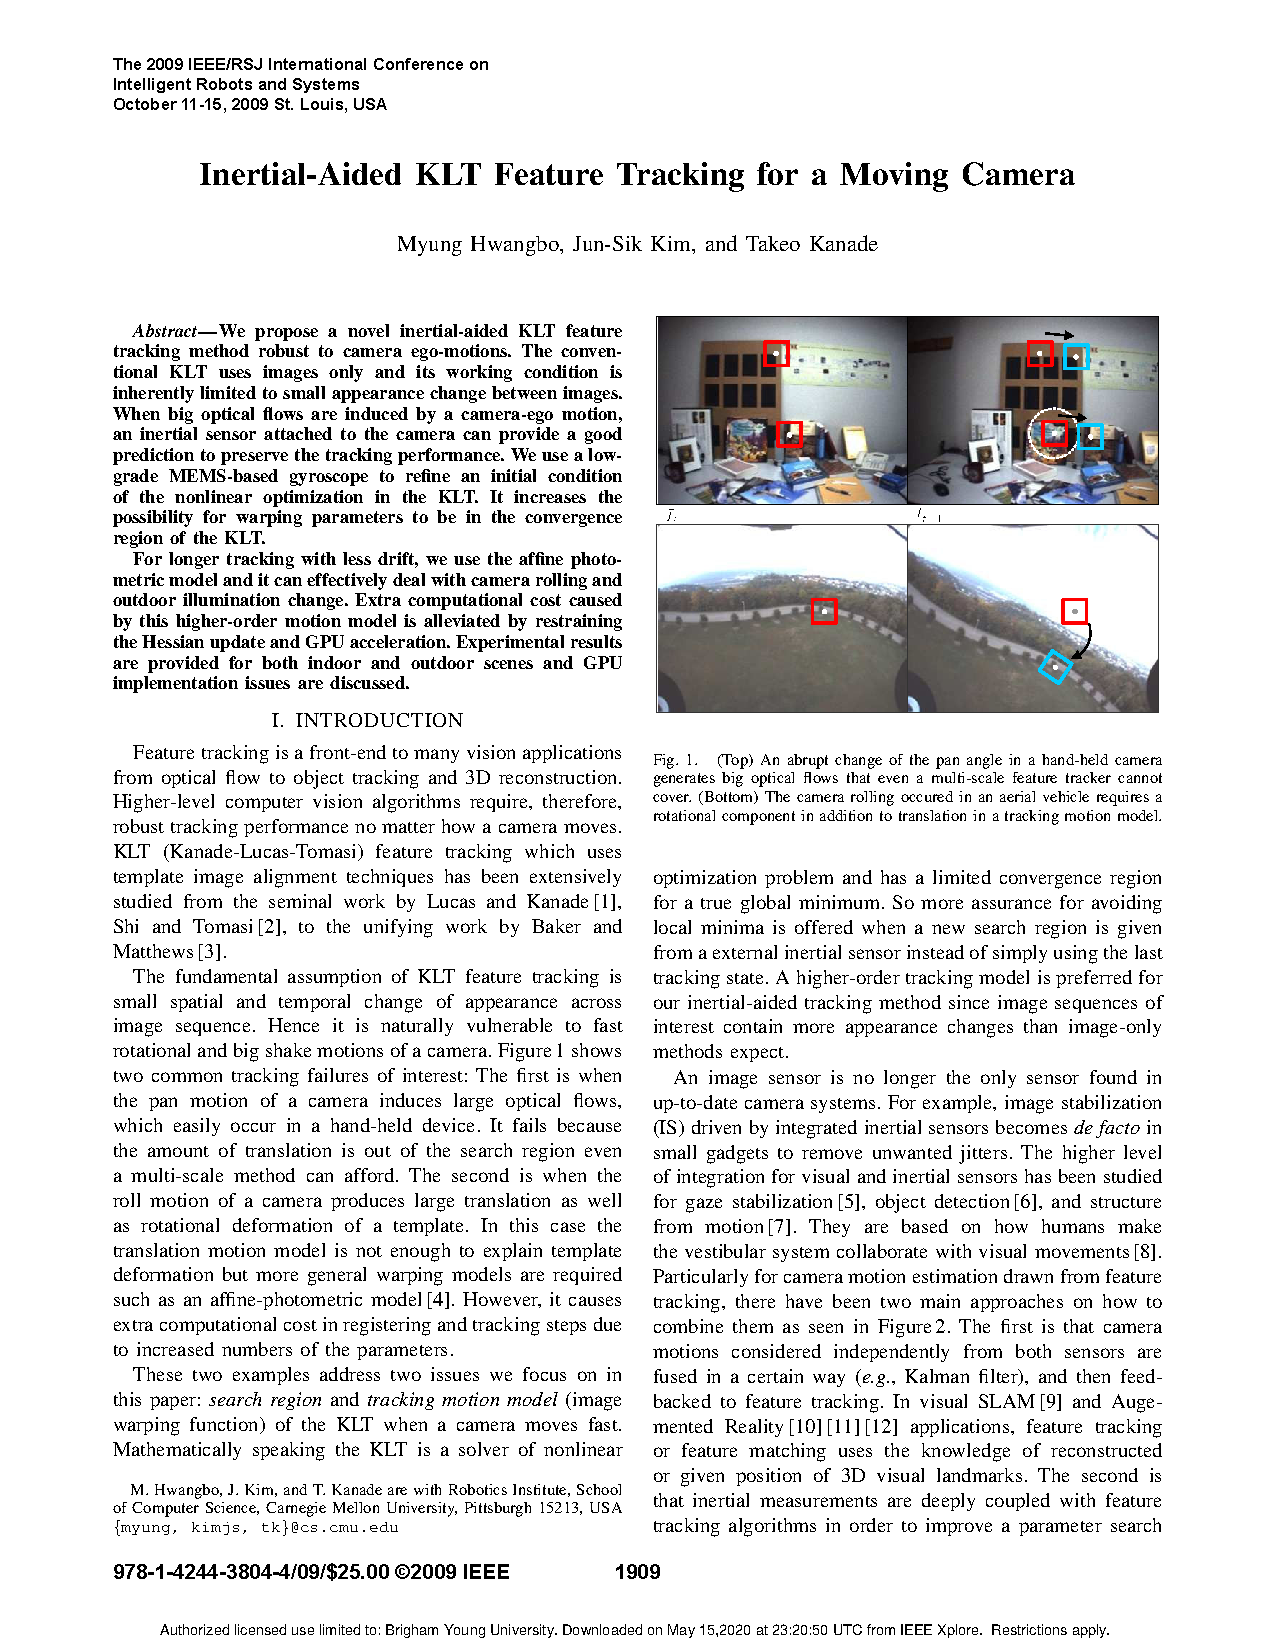
\includepdf[pages=-,scale=.8,pagecommand={}]{chap6_camera_features/papers/HwangboKimKanade09.pdf}

%------------------------------------------------------------
\section{Multirotor guidance algorithms using optical flow}
\label{sec:optical_flow_guidance}

The objective of this section is to develop guidance strategies for the multirotor that use optical flow.  The interface to the multirotor is using a velocity controller as described in Section~\ref{sec:velocity_controller}.

%-----------------------------------------------------------------
\subsection{Simple relationships between moving camera and optical flow}
\rwbcomment{I moved the more complicated relationships to the visual servoing chapter.  Could move it back here.}

We begin by deriving several relationships between a moving camera and the optical flow. 
%
Consider the picture shown in Figure~\ref{fig:optical_flow_forward_looking}, where the multirotor is moving parallel to a wall that contains features, with a front-looking camera.  
\begin{marginfigure}
	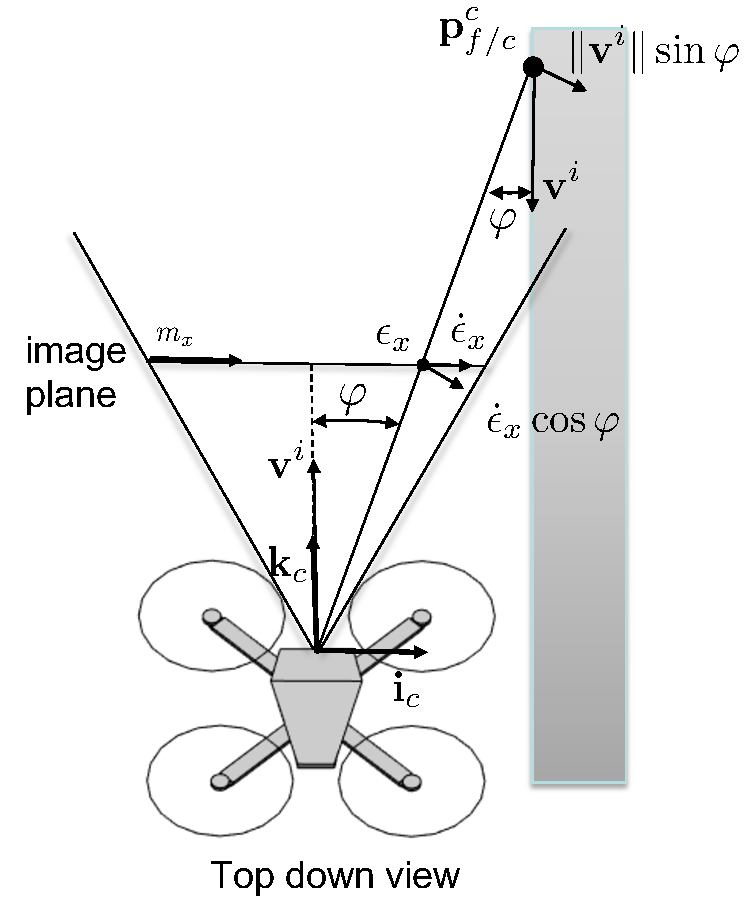
\includegraphics[width=\linewidth]{chap7_optical_flow/figures/optical_flow_forward_looking}
	\caption{Optical flow of a wall for forward looking camera.}
	\label{fig:optical_flow_forward_looking}
\end{marginfigure}
Features on the wall will move in the camera $x$-direction.
\begin{theorem}\label{thm:epsilon_x_dot_forward_looking}
	Suppose that a multirotor is moving at velocity $\mathbf{v}^i = v\kbf_c$ parallel to a wall that contains a feature at $\pbf_{f/c}^c$.  Then the calibrated optical flow of the feature in the $x$-direction is given by
	\begin{equation}\label{eq:epsilon_x_dot_forward_looking}
%	\dot{\epsilon}_x = \frac{v}{\norm{\Pi_{\ebf_3}\pbf_{f/c}^c}}\frac{\epsilon_x}{\norm{\Pi_{\ebf_3}\epsilonbf_f}},
	\dot{\epsilon}_x = \frac{v}{D}\frac{\epsilon_x}{\sqrt{\epsilon_x^2 + 1}},
	\end{equation}
	where $D$ is the distance to the feature projected on to the camera $x-z$ plane.
\end{theorem}
\begin{proof}
  The distance from the camera frame to the world feature in the horizontal plane is $D$ and the distance from the camera frame to the projection of the feature on the image plane in the horizontal plane is $d=\sqrt{\epsilon_x^2+1}$.
	From Figure~\ref{fig:optical_flow_forward_looking} we see that
	\[
	\dot{\varphi} = \frac{\dot{\epsilon}_x}{d\cos\varphi} = \frac{v\sin\varphi}{D}.
	\]
	Therefore
	\[
	\dot{\epsilon}_x = \frac{d v \cos\varphi \sin\varphi}{D}.
	\]
	Since the distance from the camera center to the image plane is equal to one, we have that $\cos\varphi = 1/d$ and $\sin\varphi = \epsilon_x/d$.  Therefore
	\[
	\dot{\epsilon}_x = \frac{v \epsilon_x}{D d}=\frac{v \epsilon_x}{D\sqrt{\epsilon_x^2+1}}.
	\]
\end{proof}

%
Consider the picture shown in Figure~\ref{fig:optical_flow_forward_looking_ground}, where the multirotor is moving parallel to the ground that contains features, with a forward-looking camera.  
\begin{marginfigure}
	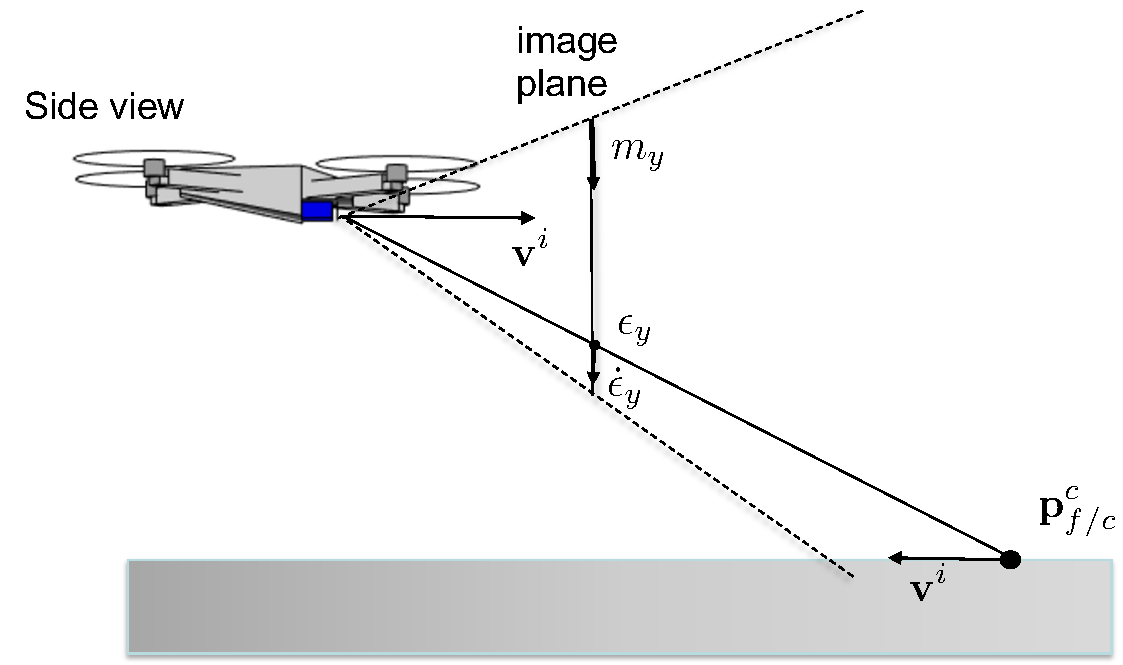
\includegraphics[width=\linewidth]{chap7_optical_flow/figures/optical_flow_forward_looking_ground}
	\caption{Optical flow of a feature on the ground for forward looking camera.}
	\label{fig:optical_flow_forward_looking_ground}
\end{marginfigure}
Features on the ground will move in the camera $y$-direction.  
\begin{theorem} \label{thm:epsilon_y_dot_forward_looking}
	Suppose that a multirotor is moving at velocity $\mathbf{v}^i = v\kbf_c$ parallel to the ground that contains a feature at $\pbf_{f/c}^c$.  Then the calibrated optical flow of the feature in the $y$-direction is given by
	\begin{equation}\label{eq:epsilon_y_dot_forward_looking}
	\dot{\epsilon}_y = \frac{v}{D}\frac{\epsilon_y}{\sqrt{\epsilon_y^2+1}},
	\end{equation}
	where $D$ is the distance to the feature projected on to the camera $y-z$ plane.
\end{theorem}
\begin{proof}
Similar to the proof of Theorem~\ref{thm:epsilon_x_dot_forward_looking}.
\end{proof}

%
Consider the picture shown in Figure~\ref{fig:optical_flow_time_to_collision}, where the multirotor is moving toward a flat wall that contains features, with a forward-looking camera.  Define the {\em time-to-collision $\tau_c$} to be the time that it will take for the multirotor to intersect the wall.
\begin{marginfigure}
	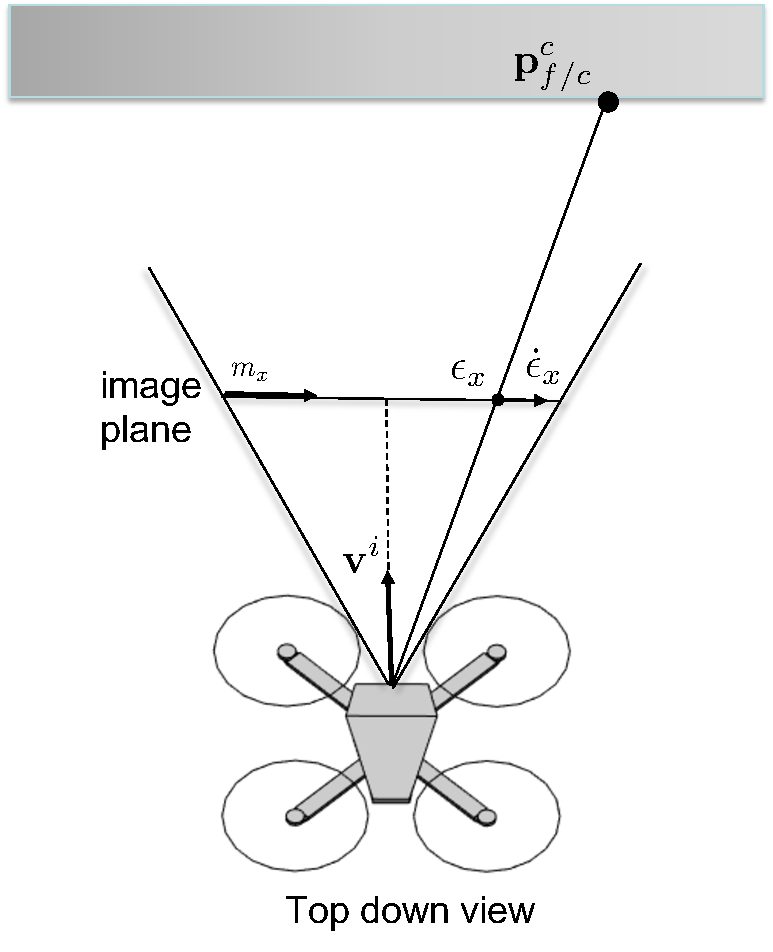
\includegraphics[width=\linewidth]{chap7_optical_flow/figures/optical_flow_time_to_collision}
	\caption{Optical flow of a feature on a wall for forward looking camera.}
	\label{fig:optical_flow_time_to_collision}
\end{marginfigure}  
\begin{theorem}
	Suppose that a multirotor is moving at velocity $\mathbf{v}^i = v\kbf_c$ and let $\mathbb{P}$ be the plane in $\mathbb{R}^3$ with normal vector $\kbf_c$ that contains a feature $\pbf_{f/c}^c$, and let $\tau_c$ be the time at which the multirotor will intersect $\mathbb{P}$.  Then if $\pbf_{f/c}^c$ is not on the ray defined by $\kbf_c$, then
	\begin{equation}\label{eq:optical_flow_time_to_collision}
	\tau_c = \frac{\epsilon_x}{\dot{\epsilon}_x} =  \frac{\epsilon_y}{\dot{\epsilon}_y}.
	\end{equation}
\end{theorem}
\begin{proof}
	Let $\pbf_{f/c}^c = (p_x, p_y, p_z)^\top$.  Then the calibrated pixel in the $x$-direction is given by
	\[
	\epsilon_x = \frac{p_x}{p_z}.
	\]
	Differentiating we get
	\begin{align}
	\dot{\epsilon}_x &= \frac{p_z\dot{p}_x - p_x\dot{p}_z}{p_z^2} \notag \\
		&= -\frac{p_x}{p_z}\left(\frac{\dot{p}_z}{p_z}\right) \\
		&= -\epsilon_x \frac{\dot{p}_z}{p_z}
		\label{eq:optical_flow_time_to_collision_1}
	\end{align}
	where the second line follows from the fact that the object does not move perpendicular to the motion, i.e., $\dot{p}_x = 0$.  Similarly it can be shown that
	\[
	\dot{\epsilon}_y = -\epsilon_y \frac{\dot{p}_z}{p_z}
	\]
	
	The time-to-collision will be the distance to the plane divided by the closing velocity, i.e., 
	\[
	\tau_c = -\frac{p_z}{\dot{p}_z},
	\]
	where we note that $\dot{p}_z$ is negative since $p_z$ is decreasing.
	Equation~\eqref{eq:optical_flow_time_to_collision} follows from Equation~\eqref{eq:optical_flow_time_to_collision_1}.
\end{proof}

If instead of tracking feature points, the computer vision algorithm tracks the area of an object, then time to collision with the plane containing the object can also be computed as shown in the next theorem.

\begin{marginfigure}
	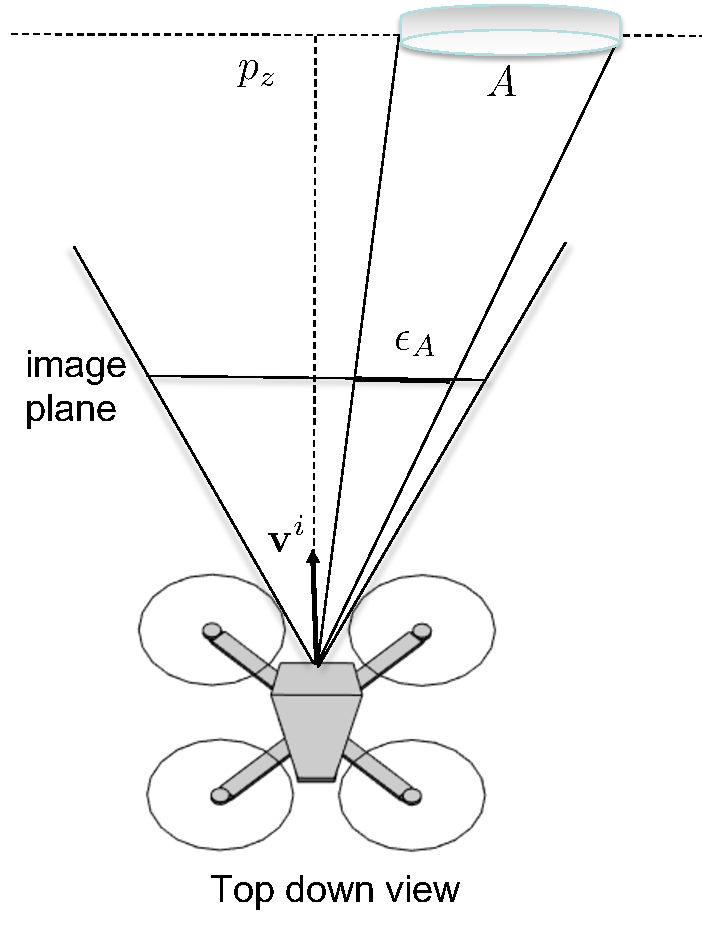
\includegraphics[width=\linewidth]{chap7_optical_flow/figures/optical_flow_time_to_collision_area}
	\caption{Time-to-collision calculation for an object with area $A$}
	\label{fig:optical_flow_time_to_collision_area}
\end{marginfigure}  
\begin{theorem}
	Suppose that a multirotor is moving at velocity $\mathbf{v}^i = v\kbf_c$ toward a plane defined by the normal vector $\kbf_c$, that contains an object of area $A$.  Let $\epsilon_A$ be the calibrated pixel area on the image plane, and let $\dot{\epsilon}_A$ be the expansion rate of the pixel area.  Then the time-to-collision with the plane containing the object is
	\begin{equation}\label{eq:optical_flow_time_to_collision_area}
	\tau_c = \frac{\epsilon_A}{\dot{\epsilon}_A}.
	\end{equation}
\end{theorem}
\begin{proof}
	The pixel area is given by
	\[
	\frac{\epsilon_A}{1} = \frac{A}{p_z}.
	\]
	Differentiating we get
	\begin{align*}
	\dot{\epsilon}_A &= -\frac{A}{p_z}\left(\frac{\dot{p}_z}{p_z}\right) \\
	&= -\epsilon_A \frac{\dot{p}_z}{p_z}.
	\end{align*}
	Therefore, the time-to-collision is
	\[
	\tau_c = -\frac{p_z}{\dot{p}_z} = \frac{\epsilon_A}{\dot{\epsilon}_A}.
	\]
\end{proof}

\begin{marginfigure}
	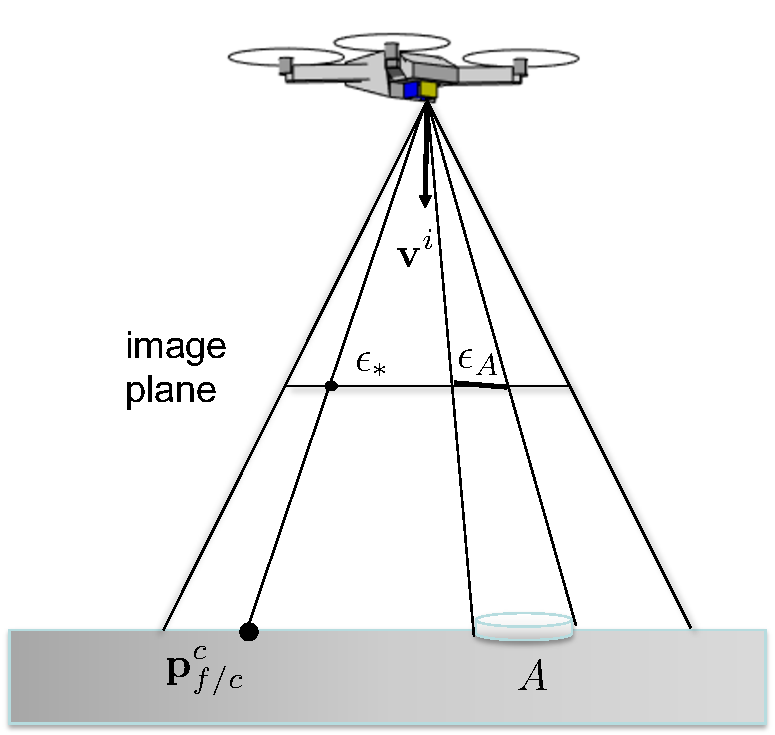
\includegraphics[width=\linewidth]{chap7_optical_flow/figures/optical_flow_time_to_land}
	\caption{Time-to-land calculation.}
	\label{fig:optical_flow_time_to_land}
\end{marginfigure}  
An obvious extension of the previous to theorems is the following corollary.
\begin{corollary}\label{cor:optical_flow_time_to_land}
	With reference to Figure~\ref{fig:optical_flow_time_to_land} suppose that a multirotor is moving with velocity $\vbf^i = v\kbf_c^i=v\kbf_b^i$ with a downward looking camera, and suppose that it is tracking either a feature at $\pbf_{f/c}^c$ that is not on the optical axis, or an area $A$, both on a horizontal ground plane, then the time-to-land is given by
	\[
	\tau_L = \frac{\epsilon_A}{\dot{\epsilon}_A} = \frac{\epsilon_x}{\dot{\epsilon}_x} = \frac{\epsilon_y}{\dot{\epsilon}_y}.
	\]
\end{corollary}
Note that if $e_A[k]$ is the area of the object in frame $k$, then 
\[
\dot{e}_A \approx \frac{e_A[k]-e_A[k-1]}{T_s},
\]
where $T_s$ is the sample time between frames.  Then the time to collision at frame $k$ can be approximated as
\[
\tau_c[k] \approx T_s\frac{e_A[k]}{e_A[k]-e_A[k-1]}.
\]


%-----------------------------------------------------------------
\subsection{Landing strategy}
From Corollary~\ref{cor:optical_flow_time_to_land} we can derive the following landing strategy. 

Assuming a downward facing camera where $\kbf_c$ is aligned with the body $z$-axis, let the commanded velocity be given by
\[
\vbf_d^i = (\alpha \tau_L + \beta) \kbf_c^i,
\]
where $\alpha$ has units of $m/s^2$ and defines the descent rate, and $\beta$ has units of $m/s$ and defines the landing velocity when the multirotor contacts the ground.

%-----------------------------------------------------------------
\subsection{Collision avoidance strategy}


\begin{marginfigure}
	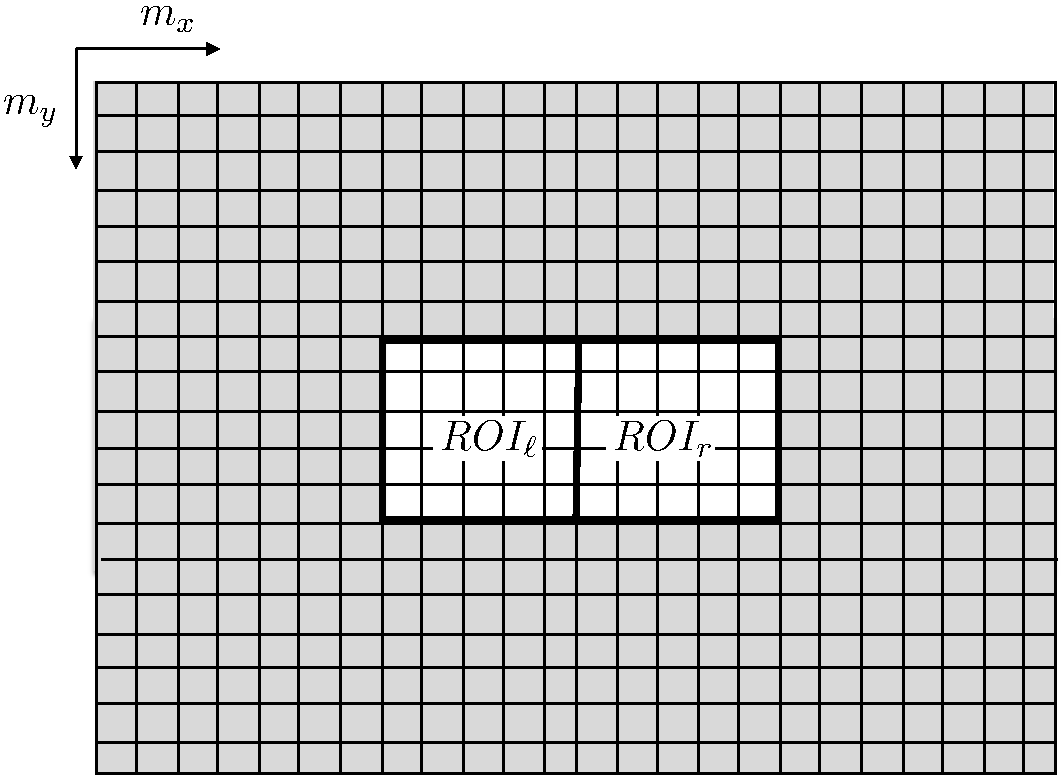
\includegraphics[width=\linewidth]{chap7_optical_flow/figures/collision_avoidance_strategy}
	\caption{Region of interest for collision avoidance.}
	\label{fig:collision_avoidance_stragegy}
\end{marginfigure}  

Consider the region of interest (ROI) shown in Figure~\ref{fig:collision_avoidance_stragegy}.

Let $\vbf_{d,nom}^i$ be a desired nominal velocity.

\begin{description}
	\item[Step 0.] Set $\vbf_d^i\leftarrow \vbf_{d,nom}^i$.
	\item[Step 1.] Find \texttt{goodFeaturesToTrack} in ROI and compute optical flow at those features.
	\item[Step 2.]  Compute time-to-collision for all features in the ROI, and find feature $\epsilonbf_{\text{min}}$ with smallest time-to-collision, $\tau_{\text{min}}$.
	\item[Step 3.]
	If $\tau_{\text{min}}<\tau_{\text{threshold}}$ and  $\epsilonbf_{\text{min}}\in ROI_r$, set
	\[
	\vbf_d^i \leftarrow \vbf_{d,nom}^i - v_s \jbf_b^i.
	\]
	If $\tau_{\text{min}}<\tau_{\text{threshold}}$ and  $\epsilonbf_{\text{min}}\in ROI_\ell$, set
	\[
	\vbf_d^i \leftarrow \vbf_{d,nom}^i + v_s \jbf_b^i.
	\]
	where $v_s$ is a side velocity to avoid the obstacle.  
\end{description}

%-----------------------------------------------------------------
\subsection{Terrain following strategy}


\begin{marginfigure}
	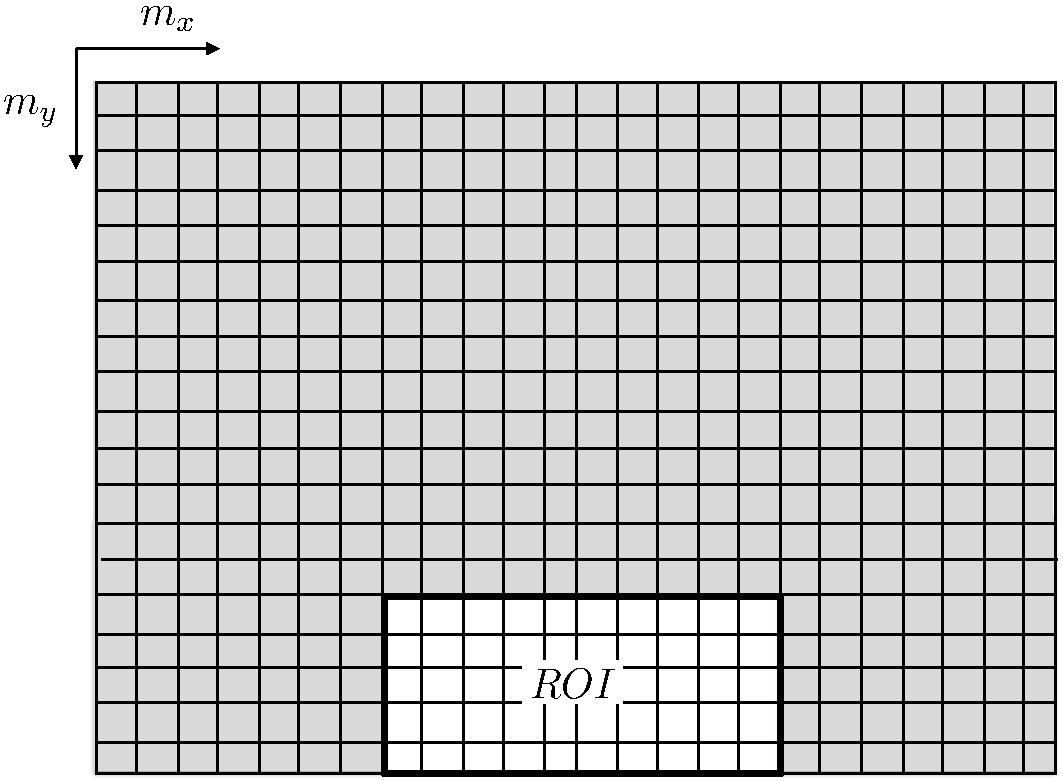
\includegraphics[width=\linewidth]{chap7_optical_flow/figures/terrain_following_strategy}
	\caption{Region of interest for terrain following.}
	\label{fig:terrain_following_stragegy}
\end{marginfigure}  

Consider the region of interest (ROI) shown in Figure~\ref{fig:terrain_following_stragegy}.


From Theorem~\ref{thm:epsilon_y_dot_forward_looking} we have seen that 
\[
	\dot{\epsilon}_y = \frac{v}{D}\frac{\epsilon_y}{\sqrt{\epsilon_y^2+1}}.
\]
where $D$ is the distance to feature in the camera $x-y$ plane.  Therefore
\[
\frac{D}{v} = \frac{\epsilon_y}{\dot{\epsilon}_y\sqrt{\epsilon_y^2+1}}.
\]
The idea with terrain following is to regulate this value to some constant $(D/v)_d$. When $v$ increases, multirotor will rise, when $v$ decreases, multirotor will descend.  If $v$ is known, then we could regulate $D$ directly.  

\begin{description}
	\item[Step 1.] Find \texttt{goodFeaturesToTrack} in ROI and compute optical flow at those features.
	\item[Step 1.]  Compute the average $D/v$ as
		\[
		\left(\frac{D}{v}\right)_{\text{ave}} = \sum_{\epsilonbf\in ROI} \frac{\epsilon_y}{\dot{\epsilon}_y\sqrt{\epsilon_y^2+1}}
		\]
	\item[Step 2.] Adjust the desired velocity as
		\[
		\vbf_d^i \leftarrow \vbf_{d,nom}^i - k\left[\left(\frac{D}{v}\right)_d - \left(\frac{D}{v}\right)_{\text{ave}}\right] \kbf_b^i,
		\]
		where $k>0$ is a tunable control gain.
\end{description}

%-----------------------------------------------------------------
\subsection{Wall following strategy}


\begin{marginfigure}
	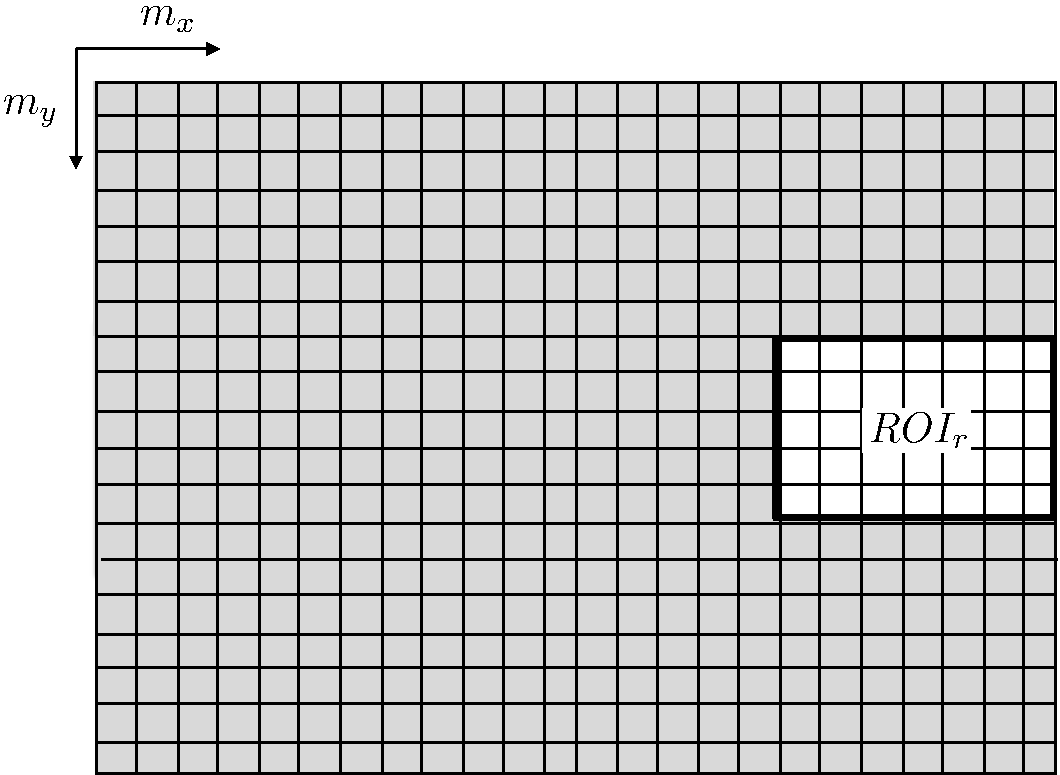
\includegraphics[width=\linewidth]{chap7_optical_flow/figures/wall_following_strategy}
	\caption{Region of interest for wall following.}
	\label{fig:wall_following_stragegy}
\end{marginfigure}  

Consider the region of interest (ROI) shown in Figure~\ref{fig:wall_following_stragegy}.


From Theorem~\ref{thm:epsilon_x_dot_forward_looking} we have seen that 
\[
\dot{\epsilon}_x = \frac{v}{D}\frac{\epsilon_x}{\sqrt{\epsilon_x^2+1}}.
\]
where $D$ is the distance to the wall feature in the camera $x-z$ plane.  Therefore
\[
\frac{D}{v} = \frac{\epsilon_x}{\dot{\epsilon}_x\sqrt{\epsilon_x^2+1}}.
\]
The idea with wall following is to regulate this value to some constant $(D/v)_d$. When $v$ increases, multirotor will move away from the wall, when $v$ decreases, the multirotor will move closer to the wall.  If $v$ is known, then we could regulate $D$ directly.  

\begin{description}
	\item[Step 1.] Find \texttt{goodFeaturesToTrack} in ROI and compute optical flow at those features.
	\item[Step 1.]  Compute the average $D/v$ as
	\[
	\left(\frac{D}{v}\right)_{\text{ave}} = \sum_{\epsilonbf\in ROI_r} \frac{\epsilon_x}{\dot{\epsilon}_x\sqrt{\epsilon_x^2+1}}
	\]
	\item[Step 2.] Adjust the desired velocity as
	\[
	\vbf_d^i \leftarrow \vbf_{d,nom}^i - k\left[\left(\frac{D}{v}\right)_d - \left(\frac{D}{v}\right)_{\text{ave}}\right] \jbf_b^i,
	\]
	where $k>0$ is a tunable control gain.
\end{description}

%-----------------------------------------------------------------
\subsection{Canyon following strategy}


\begin{marginfigure}
	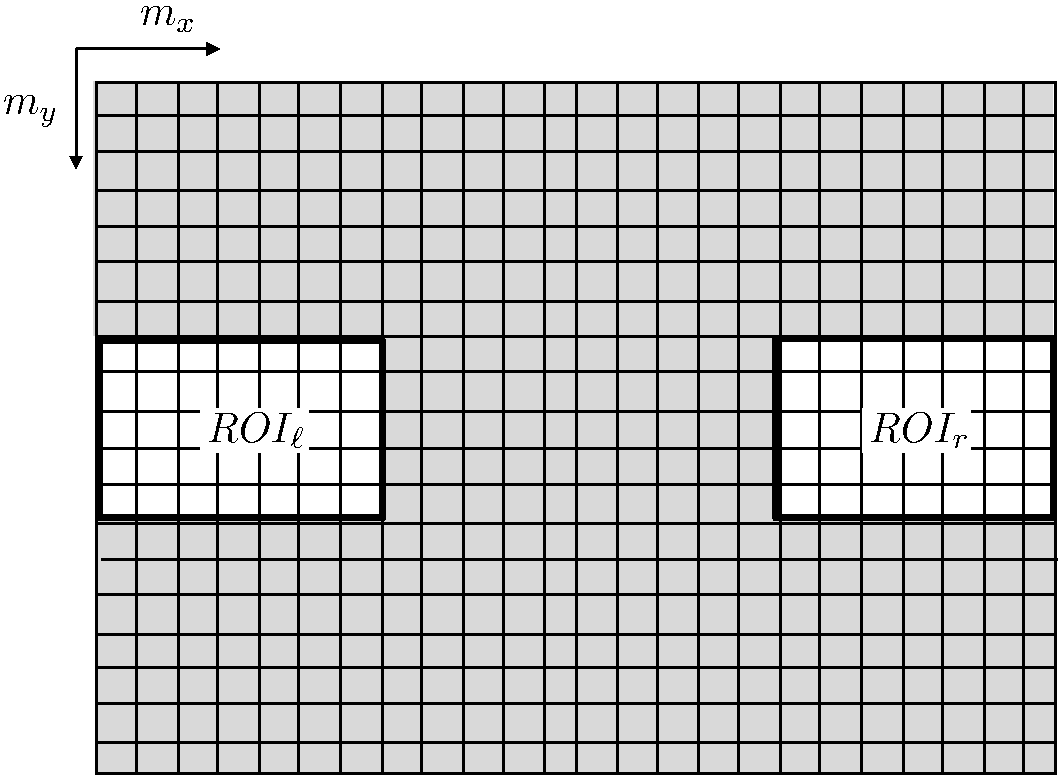
\includegraphics[width=\linewidth]{chap7_optical_flow/figures/canyon_following_strategy}
	\caption{Region of interest for canyon following.}
	\label{fig:canyon_following_stragegy}
\end{marginfigure}  

Consider the region of interest (ROI) shown in Figure~\ref{fig:canyon_following_stragegy}.

The idea is to balance the average optical flow in $ROI_\ell$ and $ROI_r$.

\begin{description}
	\item[Step 1.] Find \texttt{goodFeaturesToTrack} in $ROI_\ell$ and $ROI_r$ and compute optical flow at those features.
	\item[Step 1.]  Compute the average optical flow in each region
	\begin{align*}
		\dot{\epsilonbf}_{\ell,\text{ave}} &= \frac{1}{N}\sum_{\epsilonbf\in ROI_\ell} \dot{\epsilonbf} \\
		\dot{\epsilonbf}_{r,\text{ave}} &= \frac{1}{N}\sum_{\epsilonbf\in ROI_r} \dot{\epsilonbf},
	\end{align*}
	where $N$ is the number of pixels in $ROI$.
	\item[Step 2.] Adjust the desired velocity as
	\[
	\vbf_d^i \leftarrow \vbf_{d,nom}^i + k\left[\frac{\norm{\dot{\epsilonbf}_{\ell,\text{ave}}}-\norm{\dot{\epsilonbf}_{r,\text{ave}}}}{\norm{\dot{\epsilonbf}_{\ell,\text{ave}}}+\norm{\dot{\epsilonbf}_{r,\text{ave}}}}\right] \jbf_b^i,
	\]
	where $k$ is a control gain.
\end{description}

\section{Fly-Inspired Visual Steering of an Ultralight Indoor Aircraft, TRO, 2006}
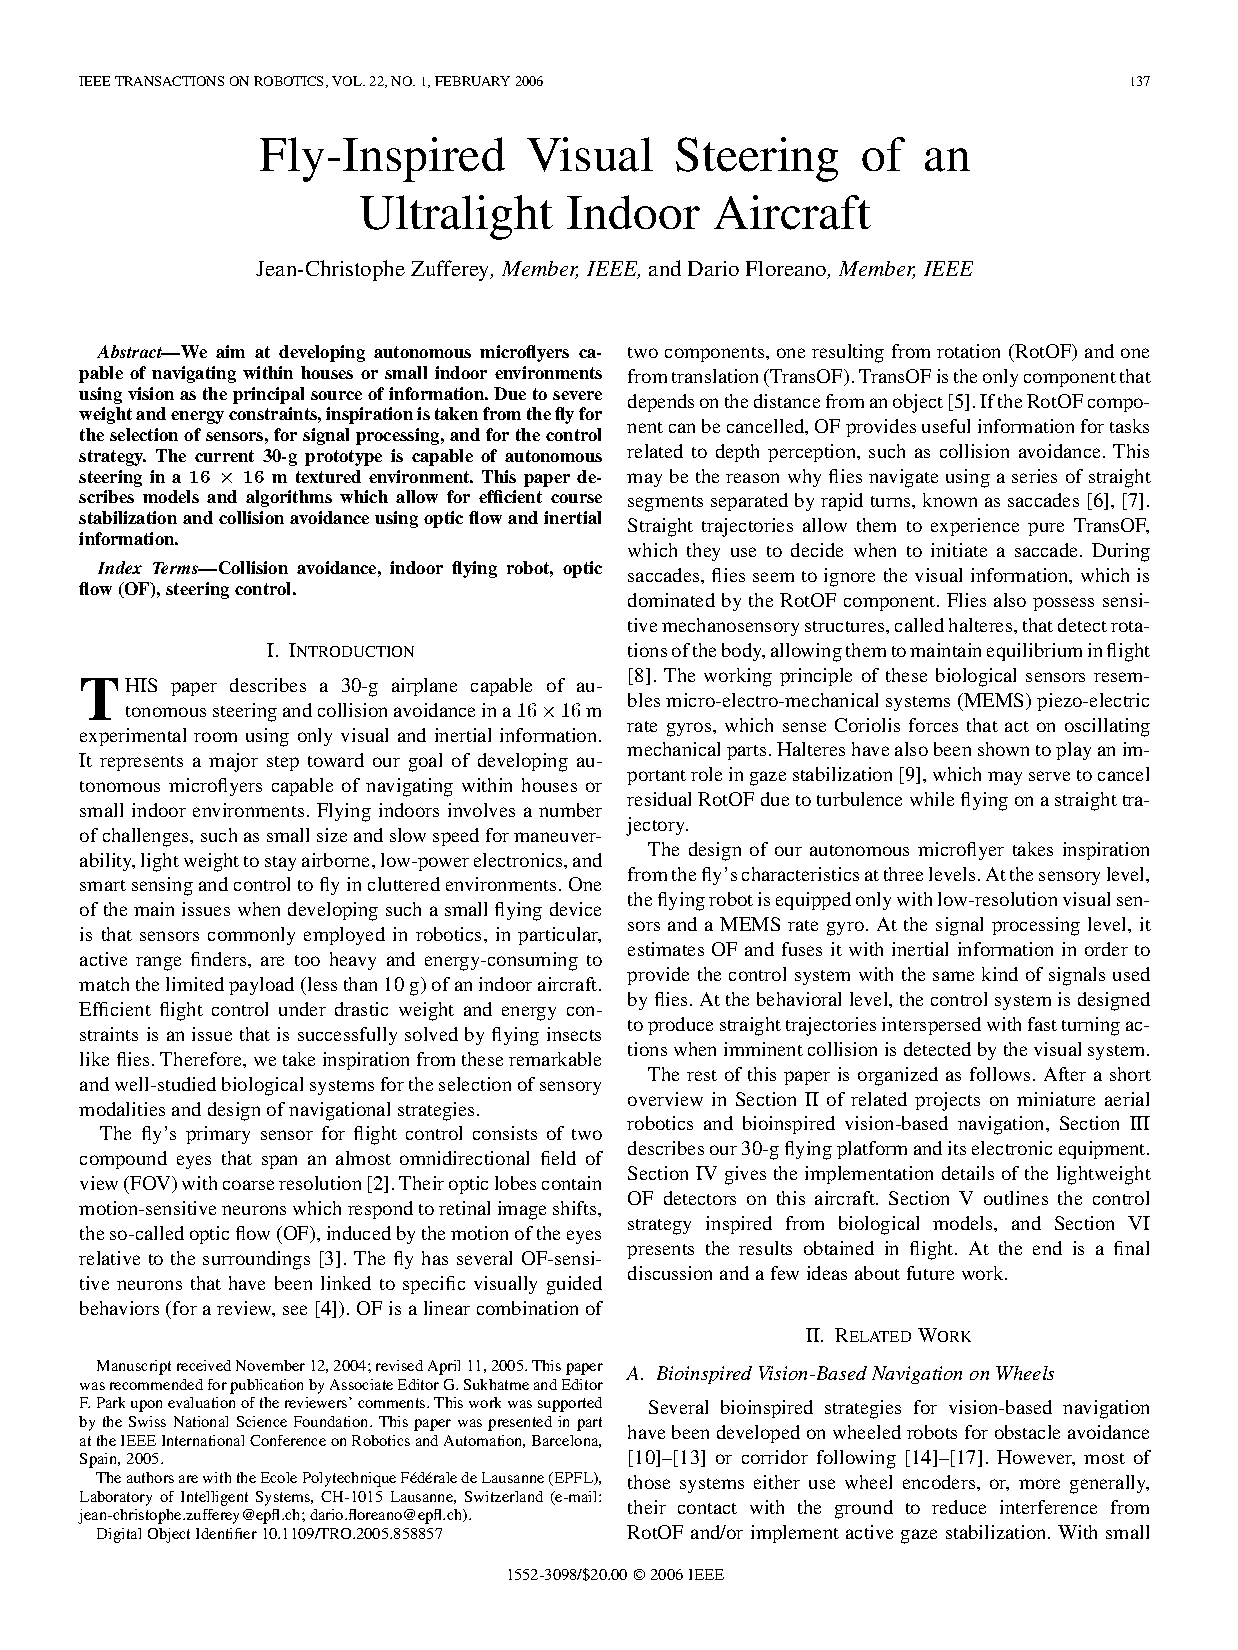
\includepdf[pages=-,scale=.8,pagecommand={}]{chap7_optical_flow/papers/ZuffereyFloreano06.pdf}


%%------------------------------------------------------------
%\subsection{Optic Flow Guidance through canyons}
%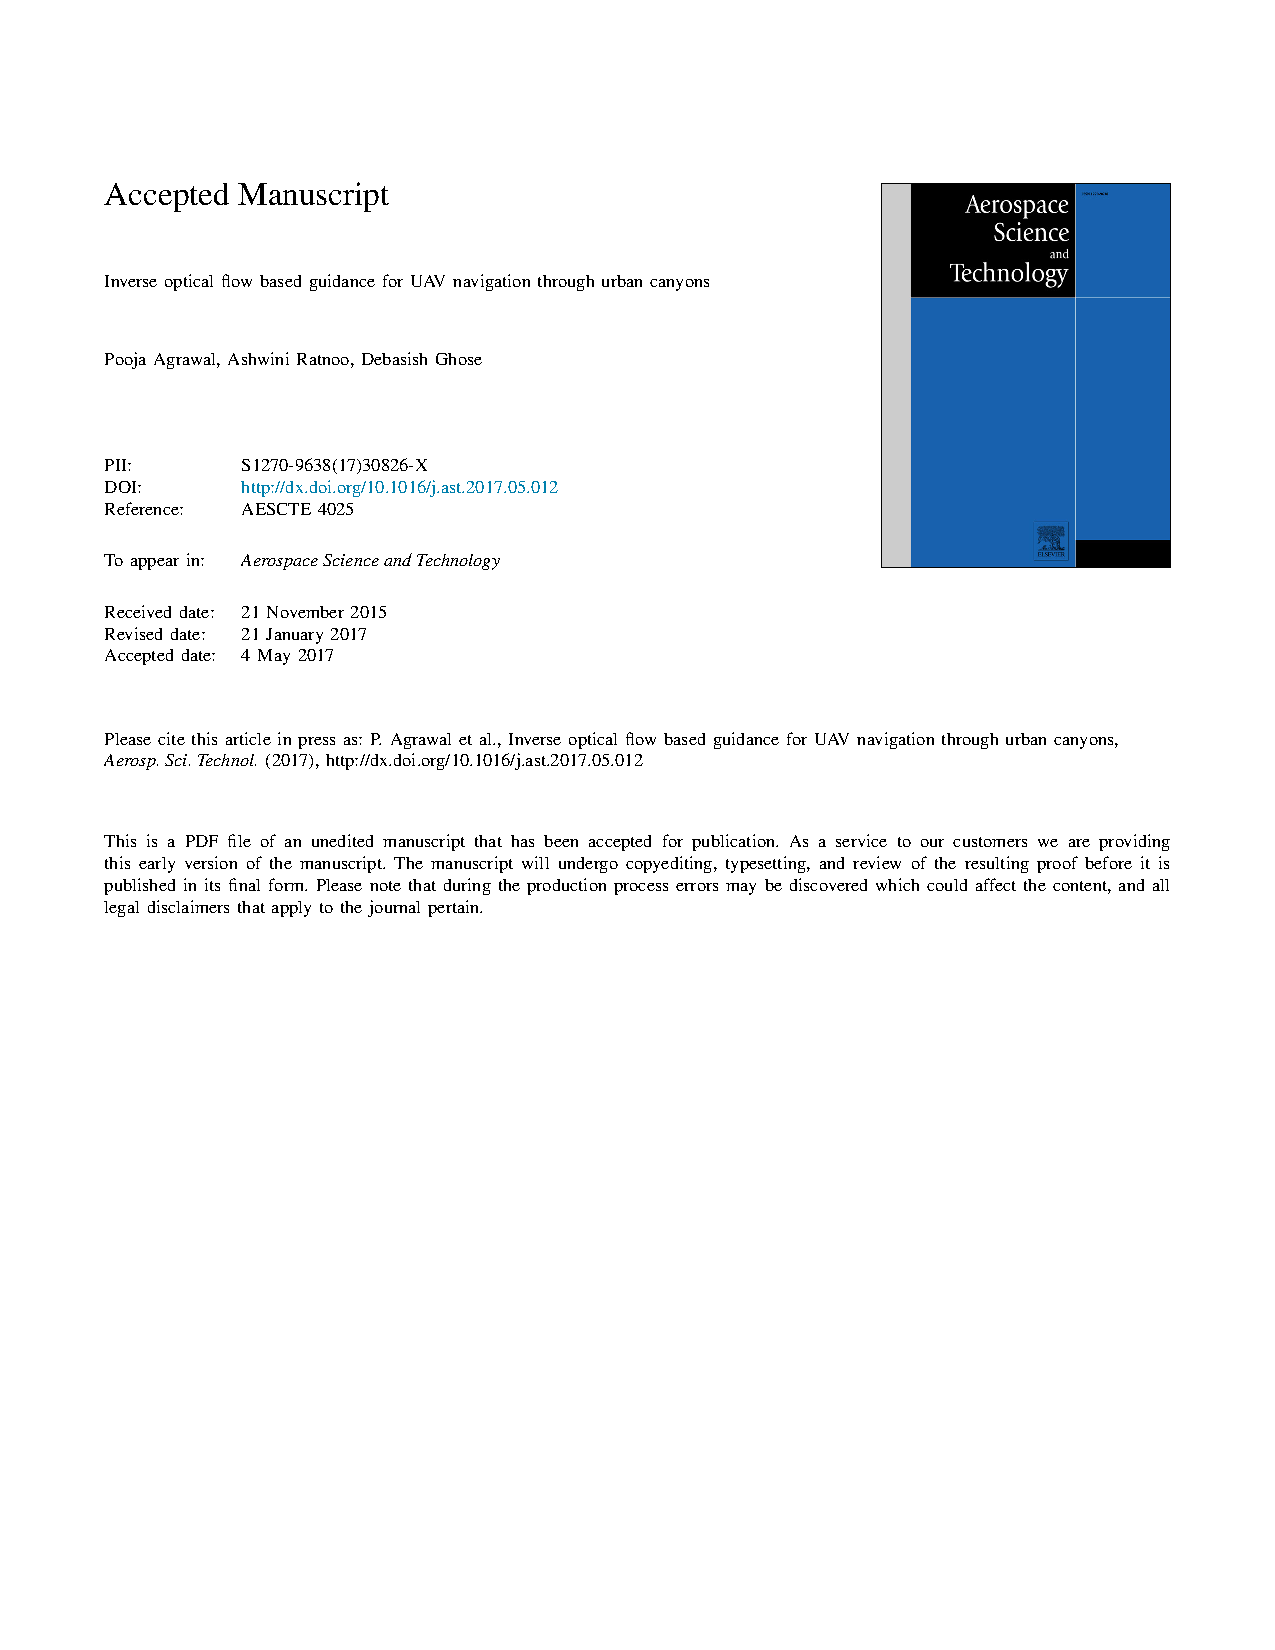
\includepdf[pages=-,scale=.8,pagecommand={}]{chap7_optical_flow/papers/AgrawalRatnooGhose17.pdf}
%
%%------------------------------------------------------------
%\subsection{Landing on boat using optic flow}
%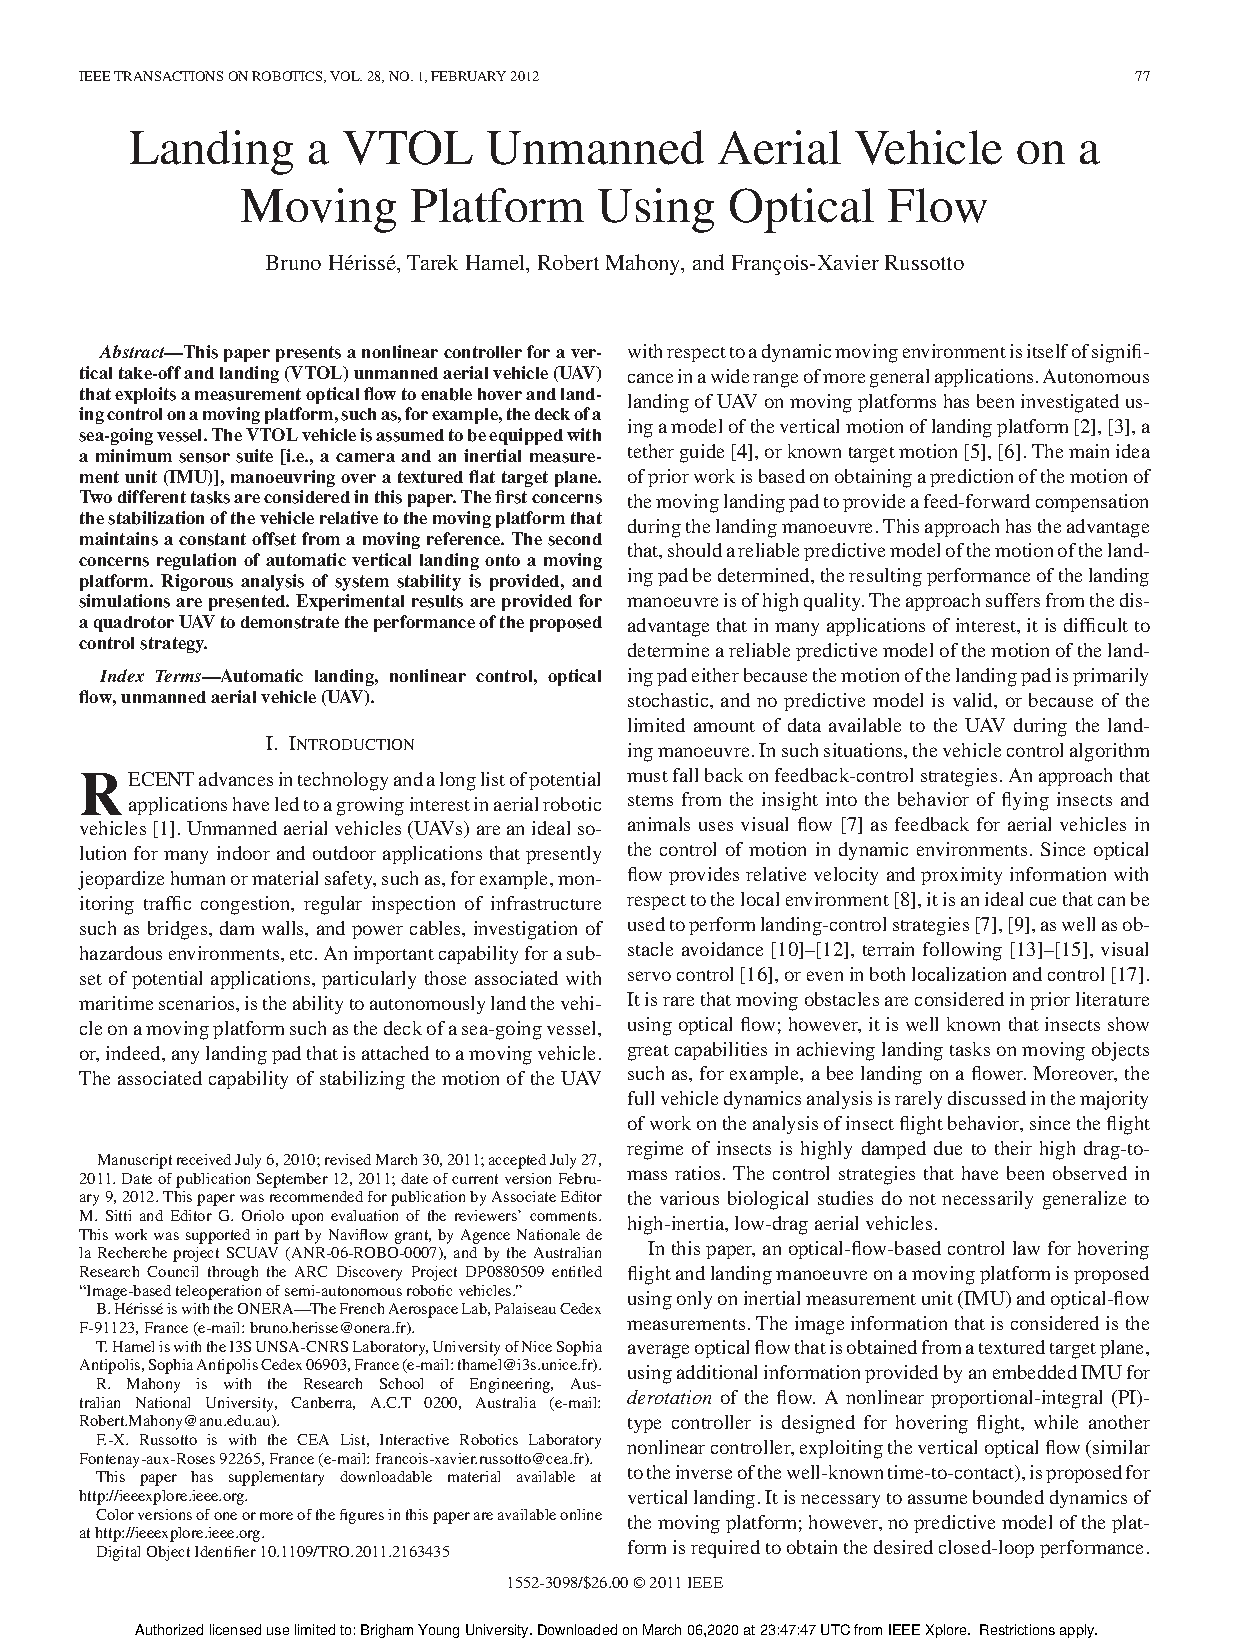
\includepdf[pages=-,scale=.8,pagecommand={}]{chap7_optical_flow/papers/HerisseHamelMahony12.pdf}







